\documentclass[11pt]{article}
\usepackage{lscape}
\usepackage{answers}
\usepackage{setspace}
\usepackage{graphicx}
\usepackage{enumitem}
\usepackage{multicol}
\usepackage{mathrsfs}
\usepackage[margin=1in]{geometry} 
\usepackage{amsmath,amsthm,amssymb}
 
\newcommand{\N}{\mathbb{N}}
\newcommand{\Z}{\mathbb{Z}}
\newcommand{\C}{\mathbb{C}}
\newcommand{\R}{\mathbb{R}}

\usepackage{hyperref}

\usepackage{booktabs}

\DeclareMathOperator{\sech}{sech}
\DeclareMathOperator{\csch}{csch}

\renewcommand{\thefigure}{S\arabic{figure}}
\renewcommand{\thetable}{S\arabic{table}}

\usepackage[numbers,compress,super]{natbib}
 
\newenvironment{theorem}[2][Theorem]{\begin{trivlist}
\item[\hskip \labelsep {\bfseries #1}\hskip \labelsep {\bfseries #2.}]}{\end{trivlist}}
\newenvironment{definition}[2][Definition]{\begin{trivlist}
\item[\hskip \labelsep {\bfseries #1}\hskip \labelsep {\bfseries #2.}]}{\end{trivlist}}
\newenvironment{proposition}[2][Proposition]{\begin{trivlist}
\item[\hskip \labelsep {\bfseries #1}\hskip \labelsep {\bfseries #2.}]}{\end{trivlist}}
\newenvironment{lemma}[2][Lemma]{\begin{trivlist}
\item[\hskip \labelsep {\bfseries #1}\hskip \labelsep {\bfseries #2.}]}{\end{trivlist}}
\newenvironment{exercise}[2][Exercise]{\begin{trivlist}
\item[\hskip \labelsep {\bfseries #1}\hskip \labelsep {\bfseries #2.}]}{\end{trivlist}}
\newenvironment{solution}[2][Solution]{\begin{trivlist}
\item[\hskip \labelsep {\bfseries #1}]}{\end{trivlist}}
\newenvironment{problem}[2][Problem]{\begin{trivlist}
\item[\hskip \labelsep {\bfseries #1}\hskip \labelsep {\bfseries #2.}]}{\end{trivlist}}
\newenvironment{question}[2][Question]{\begin{trivlist}
\item[\hskip \labelsep {\bfseries #1}\hskip \labelsep {\bfseries #2.}]}{\end{trivlist}}
\newenvironment{corollary}[2][Corollary]{\begin{trivlist}
\item[\hskip \labelsep {\bfseries #1}\hskip \labelsep {\bfseries #2.}]}{\end{trivlist}}

\setlength{\parindent}{0em}
\setlength{\parskip}{1em}
 
\begin{document}
 
% --------------------------------------------------------------
%                         Start here
% --------------------------------------------------------------
 
\title{Multi-omic strategies for transcriptome-wide prediction
    and association studies}
\author{Supplementary Materials} 
    \date{}
 
\maketitle

\section{Supplementary methods}

\subsection{Asymptotic test
of total mediation effect}


In DePMA, a distal-eQTL $s$
is tested for its total mediation effect on gene $G$
through $m$ mediators that are local to $s$.
Consider the following
mediation model for $1 \leq j \leq m$:

\begin{equation}\label{mediationeqn}
\begin{split}
Y_G & = X_s\beta_s + \mathbf{M}\beta_{\mathbf{M}} + \mathbf{X}_C\beta_{C} + \varepsilon_{Y_G} \\
M_j & = X_s\alpha_{M_j} + \mathbf{X}_C\alpha_{C,j} + \varepsilon_{M_j}
\end{split}
\end{equation}.

Here, we construct the total mediation effect 

$$\text{TME} = 
\alpha_{\mathbf{M}}^T\beta_{\mathbf{M}} = 
\sum_{i=1}^{m}\alpha_{M_i}\beta_{M_i}.$$

Note that $\text{TME}$ is distributed
as the product of two multivariate Normal
distributions. By the multivariate
Delta method \cite{Bishop}, we can obtain the
standard error for the estimated
$\text{TME}$. Let 
$\boldsymbol{\theta} = (\alpha_\mathbf{M},\beta_\mathbf{M})$
and define $f(\boldsymbol{\theta}) = TME = 
\sum_{i=1}^{m}\alpha_{M_i}\beta_{M_i}$.

The first order partial derivative
of $f(\hat{\boldsymbol{\theta}})$
is

$$d_{\hat{\boldsymbol{\theta}}} = \frac{\partial(\sum_{i=1}^{m}\alpha_{M_i}\beta_{M_i})}{\partial{\hat{\boldsymbol{\theta}}}} = [\beta_{\mathbf{M}}~\alpha_{\mathbf{M}}]^T.$$

We also obtain the estimated 
variance-covariance matrix $\hat{\boldsymbol{\Sigma}}$ 
of $\hat{\boldsymbol{\theta}}$:

$$ \hat{\boldsymbol{\Sigma}} = 
\begin{bmatrix}
\hat{\boldsymbol{\Sigma}}_{\alpha_\mathbf{M}} & \hat{\boldsymbol{\Sigma}}_{\alpha_\mathbf{M}\beta_\mathbf{M}} \\
\hat{\boldsymbol{\Sigma}}_{\alpha_\mathbf{M}\beta_\mathbf{M}} & \hat{\boldsymbol{\Sigma}}_{\beta_\mathbf{M}}
\end{bmatrix},$$

where $\hat{\boldsymbol{\Sigma}}_{\alpha_\mathbf{M}}, \hat{\boldsymbol{\Sigma}}_{\beta_\mathbf{M}},~\text{and}~ \hat{\boldsymbol{\Sigma}}_{\alpha_\mathbf{M}\beta_\mathbf{M}}$
are the variances and covariance of $\hat{\alpha}_{\mathbf{M}}$,
$\hat{\beta}_{\mathbf{M}}$, and between 
$\hat{\alpha}_{\mathbf{M}}$ and
$\hat{\beta}_{\mathbf{M}}$, respectively. Sobel previously
has shown, that with sufficient sample size,
$\hat{\boldsymbol{\Sigma}}_{\alpha_\mathbf{M}\beta_\mathbf{M}}
\approx 0$ \cite{Sobel1982AsymptoticModels,Sobel1987DirectModels}.
Thus, the standard error of $\hat{\boldsymbol{\theta}}$
is given by 

$$\hat{\sigma}^2_{\hat{\boldsymbol{\theta}}} = d_{\hat{\boldsymbol{\theta}}}^T\hat{\boldsymbol{\Sigma}}d_{\hat{\boldsymbol{\theta}}}.$$

We can then test $H_0:\text{TME} = 0$ against $H_1:\text{TME} \neq 0$
with the two-sided Wald-type test with the test statistic 
$Z =
\frac{\alpha_{\mathbf{M}}^T\beta_{\mathbf{M}}}{\sqrt{\hat{\sigma}^2_{\hat{\boldsymbol{\theta}}}}}$ and comparing to the null standard Normal distribution.

We illustrate the trade-off between power and computational speed
using the asymptotic Sobel test and the permutation speed.
Consider the following simulation framework with $m=5$ mediators,
3 covariates
and a sample size of $n \in \{200, 500, 700, 1000\}$
for the model in Equations \ref{mediation}:

\begin{itemize}
\item an $n$-length genotype vector for SNP
$s$ is drawn from $\text{Binomial}(2,MAF)$, where
the minor allele frequency $MAF$ is set at 0.1 in \textbf{Supplemental Figure \ref{fig:ch4_fig2}}below;
\item Under the alternative, we simulated 
$\beta_X \sim N(0,1)$,
$\beta_\mathbf{M} \sim \mathbf{N}_5(\mathbf{0},\mathbf{I}_5)$,
$\beta_C \sim \mathbf{N}_3(\mathbf{0},\mathbf{I}_3)$,
$\alpha_{M_j}|_{j=1}^{m=5} \sim N(0,1)$,
$\alpha_C \sim \mathbf{N}_5(\mathbf{0},\mathbf{I}_5)$.
\item Under the null, all regression parameters
were simulated as in the alternative case. However,
we set $\alpha_{M_j} = 0|_{j=1}^m$ and $\beta_{\mathbf{M}} = \mathbf{0}$.
\item Lastly, $\varepsilon_{Y_G} \sim N(0,1-h^2)$
and $\varepsilon_{M_j} \sim N(0,1-h^2_M)$, where
$h^2 = h^2_M = 0.1$ in \textbf{Supplemental Figure \ref{fig:ch4_fig2}} below.
\item We then constructed $Y_G$ and $\mathbf{M}$
using Equations \ref{mediation}.
\end{itemize}

We found, that over 10,000 simulations, the permutation test
was considerably more powerful, albeit considerably slower.
However, in most cases of implementing 
DePMA,
the number of tests of mediation are usually on
the order of $10^1$ to $10^2$. We recommend the permutation
test in most cases, unless gene $G$ has thousands
of identified distal-eQTLs.
Parallel implementations have
been offered as options in the MOSTWAS
package.

\pagebreak

\subsection{Added-last test of distal-SNPs}

Here, we propose a test to assess
the information added from distal-eSNPs
in the weighted burden test beyond
what we find from local SNPs.
Let $\mathbf{Z}_l$ (an $n_l$-vector) and 
$\mathbf{Z}_d$ (an $n_d$-vector) be the $Z$-scores
local and distal SNPs identified
by a MOSTWAS model, with
$\mathbf{Z} = [\mathbf{Z}_l~\mathbf{Z}_d]^T$ 
(an $n$ vector). The local
and distal SNP effects
from the MOSTWAS model are represented
in $\mathbf{w}_l$ (an $n_l$-vector) and 
$\mathbf{w}_d$ 
(an $n_d$-vector),
with $\mathbf{w} = [\mathbf{w}_l~\mathbf{w}_d]^T$ 
(an $n$ vector). Here, we are
interested in testing

$$H_0: \mathbf{w}_d^T\mathbf{Z}_d | \mathbf{w}_l^T\mathbf{Z}_l = \tilde{Z}_{l,\text{obs}} = 0,$$

where $\tilde{Z}_{l,\text{obs}}$
is the observed weighted $Z$-score
from local SNPs.

Under the null distribution, as
proposed by Pasaniuc et al and Gusev et al
in the Imp-G 
framework\cite{Pasaniuc2014FastEnrichment,Gusev2016},
we assume that $Z \sim N_n\left(\mathbf{0},\mathbf{\Sigma}\right),$
where

$$\mathbf{\Sigma} = \begin{bmatrix}
\mathbf{\Sigma}_{l} & \mathbf{\Sigma}_{l,d} \\
\mathbf{\Sigma}_{l,d}^T & \mathbf{\Sigma}_{d}
\end{bmatrix}$$

is the LD matrix for the SNPs, as estimated
from the reference panel. $\mathbf{\Sigma}_{l}$
and $\mathbf{\Sigma}_{d}$ represent
the LD matrices for local and distal SNPs,
respectively. The LD matrix
between local and distal SNPs $\mathbf{\Sigma}_{l,d}$
can be assumed to be zero, though
recent studies have showed long-range
LD in the human genome
\cite{Koch2013LongGenome,Park2019Population-specificVariants}.
We allow the user to set cross-chromosomal
LD to 0, though by default,
we estimate LD from the reference panel.

Now, we see that, under this null hypothesis,
the joint distribution of 
$(\tilde{Z}_l,\tilde{Z}_d) =
(w_l^TZ_l,w_d^TZ_d)$
is given by:

$$\begin{pmatrix}
\tilde{Z_l}  \\
\tilde{Z_d}
\end{pmatrix} \sim N_2\left(\textbf{0},
\begin{bmatrix}
w_l^T\mathbf{\Sigma}_{l}w_l & w_l^T\mathbf{\Sigma}_{l,d}w_d \\
w_d^T\mathbf{\Sigma}_{l,d}^Tw_l & w_d^T\mathbf{\Sigma}_{d}w_d
\end{bmatrix}
\right).$$

It follows that, given 
$\tilde{Z}_l = \tilde{Z}_{l,\text{obs}}$,

$$\tilde{Z}_d | \tilde{Z}_l = \tilde{Z}_{l,\text{obs}} \sim N\left(\frac{w_l^T\mathbf{\Sigma}_{l,d}w_d}{w_l^T\mathbf{\Sigma}_{l}w_l}\tilde{Z}_{l,\text{obs}},w_d^T\mathbf{\Sigma}_{d}w_d - \frac{[w_l^T\mathbf{\Sigma}_{l,d}w_d]^2}{w_l^T\mathbf{\Sigma}_{l}w_l}\right).$$

We can use this null distribution for
the one-sided test of
$H_0: \mathbf{w}_d^T\mathbf{Z}_d | \mathbf{w}_l^T\mathbf{Z}_l = \tilde{Z}_{l,\text{obs}} = 0$
against
$H_1: \mathbf{w}_d^T\mathbf{Z}_d | \mathbf{w}_l^T\mathbf{Z}_l = \tilde{Z}_{l,\text{obs}} > 0$. These test
is implemented in MOSTWAS as a follow-up
to the weighted-burden test.

\pagebreak

\section{Supplemental Tables and Figures}


\begin{table}[!h]
\centering
\begin{tabular}{@{}ccc@{}}
\multicolumn{1}{l}{} & \textbf{TCGA-BRCA} & \textbf{ROS/MAP} \\ \midrule
\textbf{Local-only} & 0.037 (0.053) & 0.079 (0.119) \\
\textbf{MeTWAS} & 0.040 (0.066) & 0.135 (0.099) \\
\textbf{DePMA} & 0.383 (0.194) & 0.405 (0.118) \\ \bottomrule
\end{tabular}
\caption{\emph{Comparison of $h^2$
across local-only,
MeTWAS, and DePMA predictive models.}
The mean and standard deviation of $h^2$
across all genes that are significantly
heritable with the genetic loci
considered in the design matrix
of each predictive model.}
\label{tbl:ch4_supptab1}
\end{table}

\begin{figure}[htbp]
\centering
	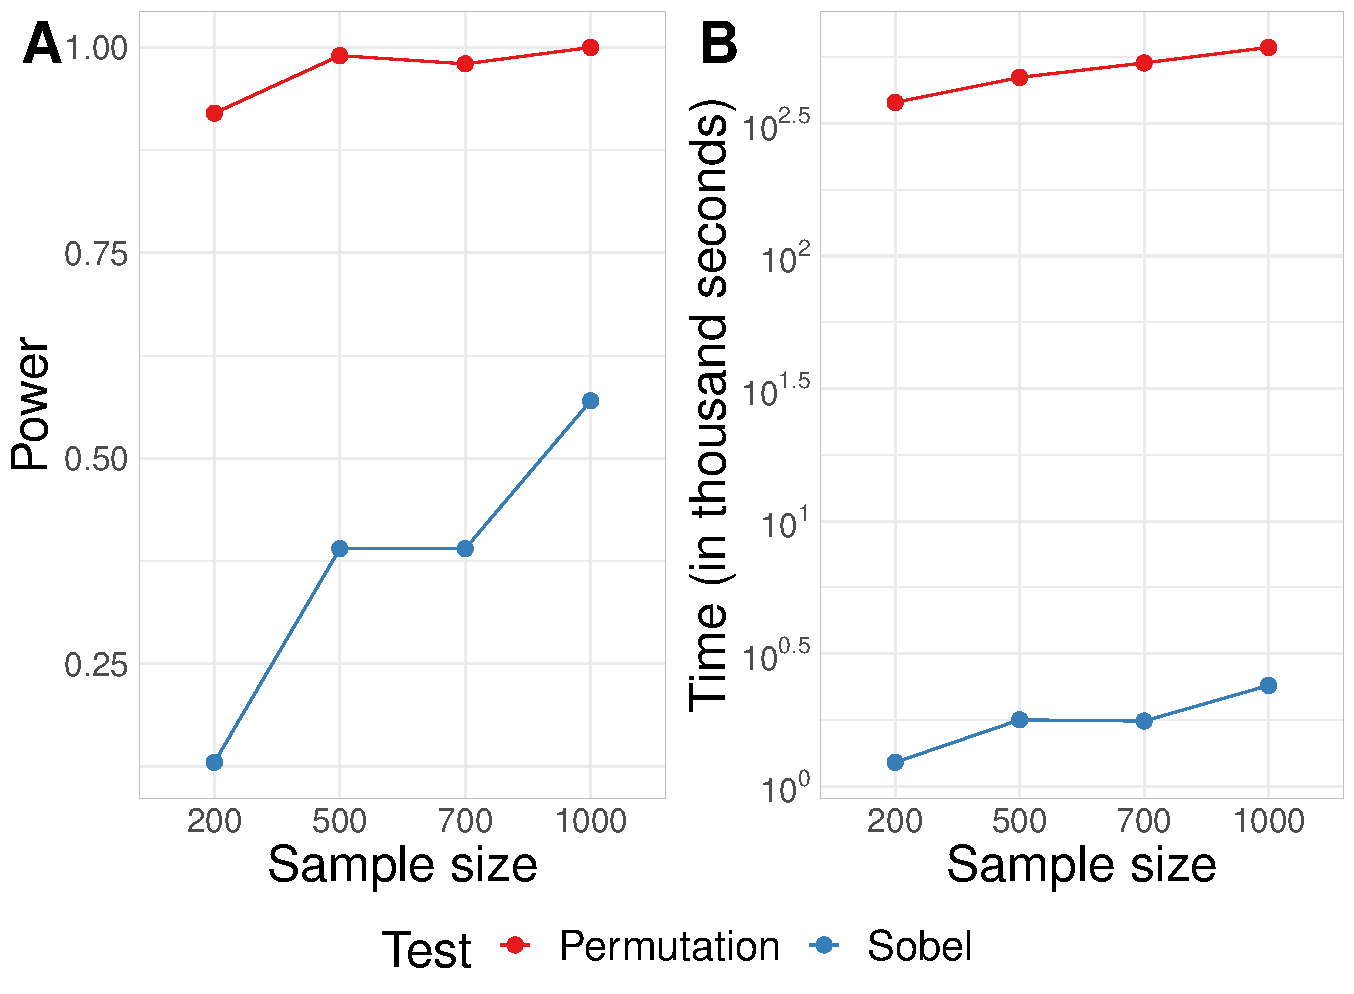
\includegraphics[width = .7\textwidth]{figures/ch4_fig2.pdf}
	\caption{\emph{Comparison of power 
	and computational speed comparison 
	of permutation and Sobel test.} Power (A) and computational speed (B) of permutation test (red)
	and asymptotic Sobel test (blue) in simulation framework}
	\label{fig:ch4_fig2}
\end{figure}

\begin{figure}[htbp]
\centering
	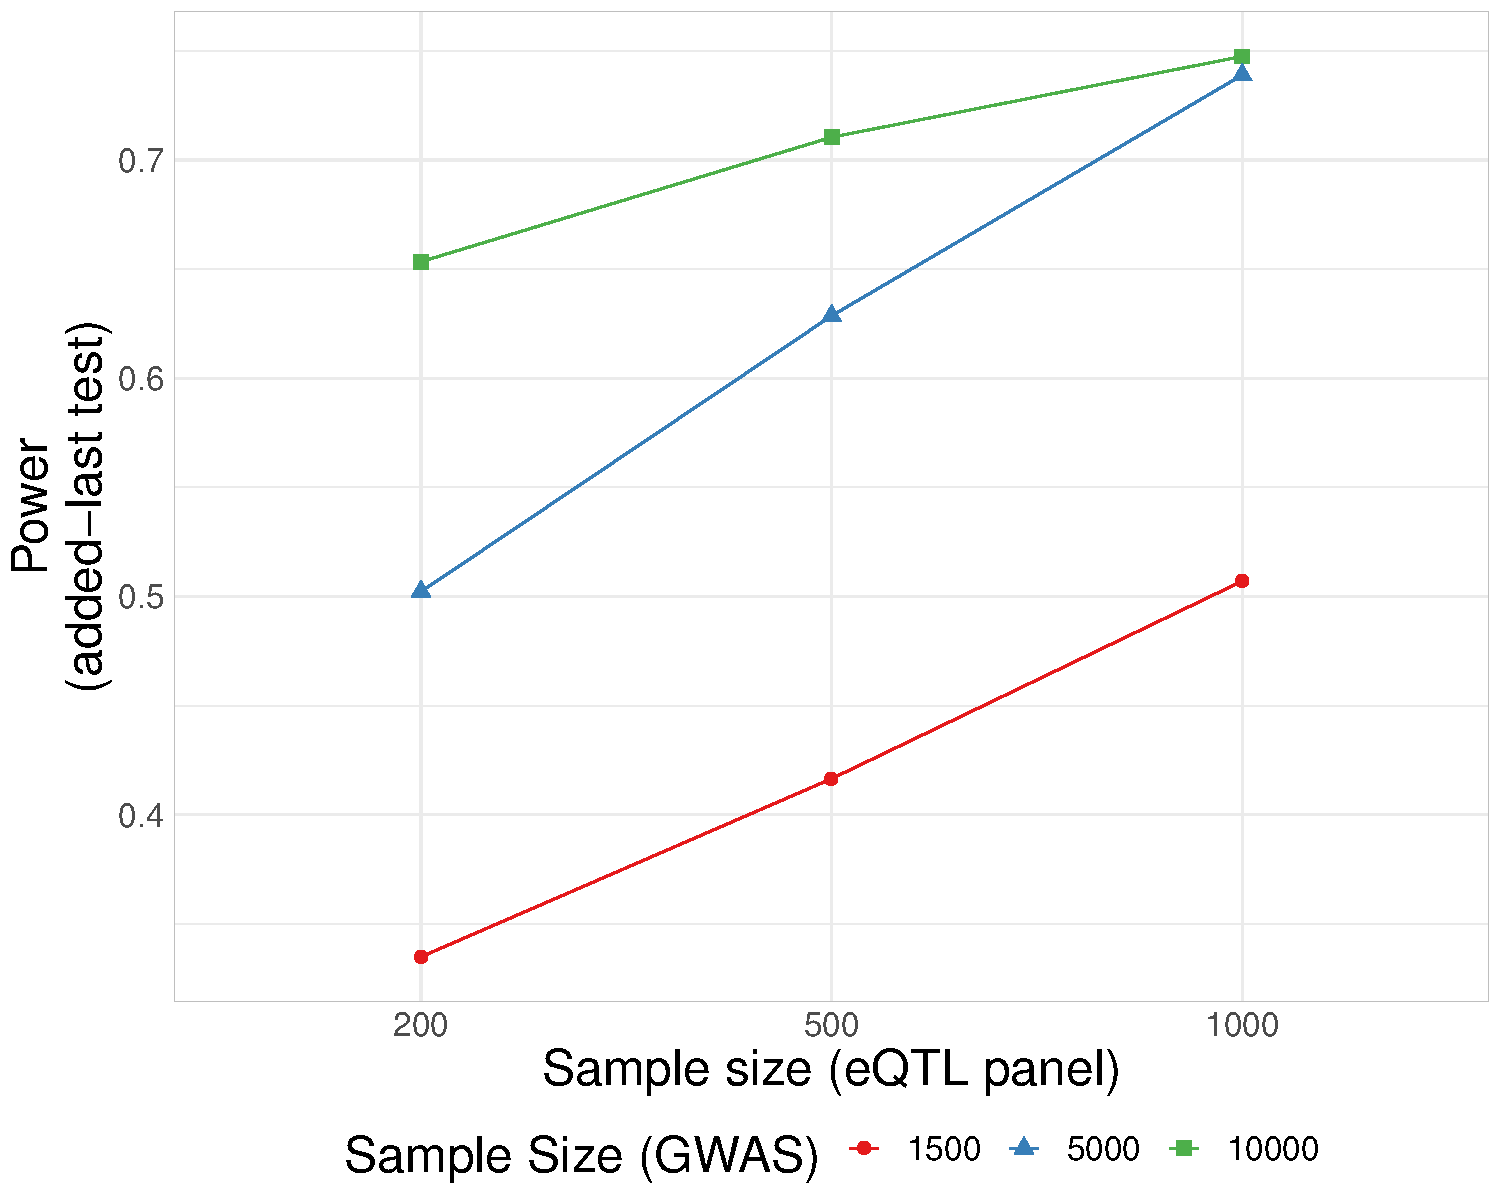
\includegraphics[width = .7\textwidth]{figures/ch4_suppfig4.pdf}
	\caption{\emph{Simulation
	analysis for the power
	of the distal variants
	added-last test.} Across
	various sample sizes
	for the eQTL reference ($X$-axis)
	panel and GWAS imputation
	panel (color), the power
	of the distal added-last
	test to detect a significant
	association with distal
	variants conditional
	on a significant local association
	at FDR-adjusted $P < 0.05$.}
	\label{fig:ch4_suppfig4}
\end{figure}

\begin{center}
\begin{figure}[!h]
    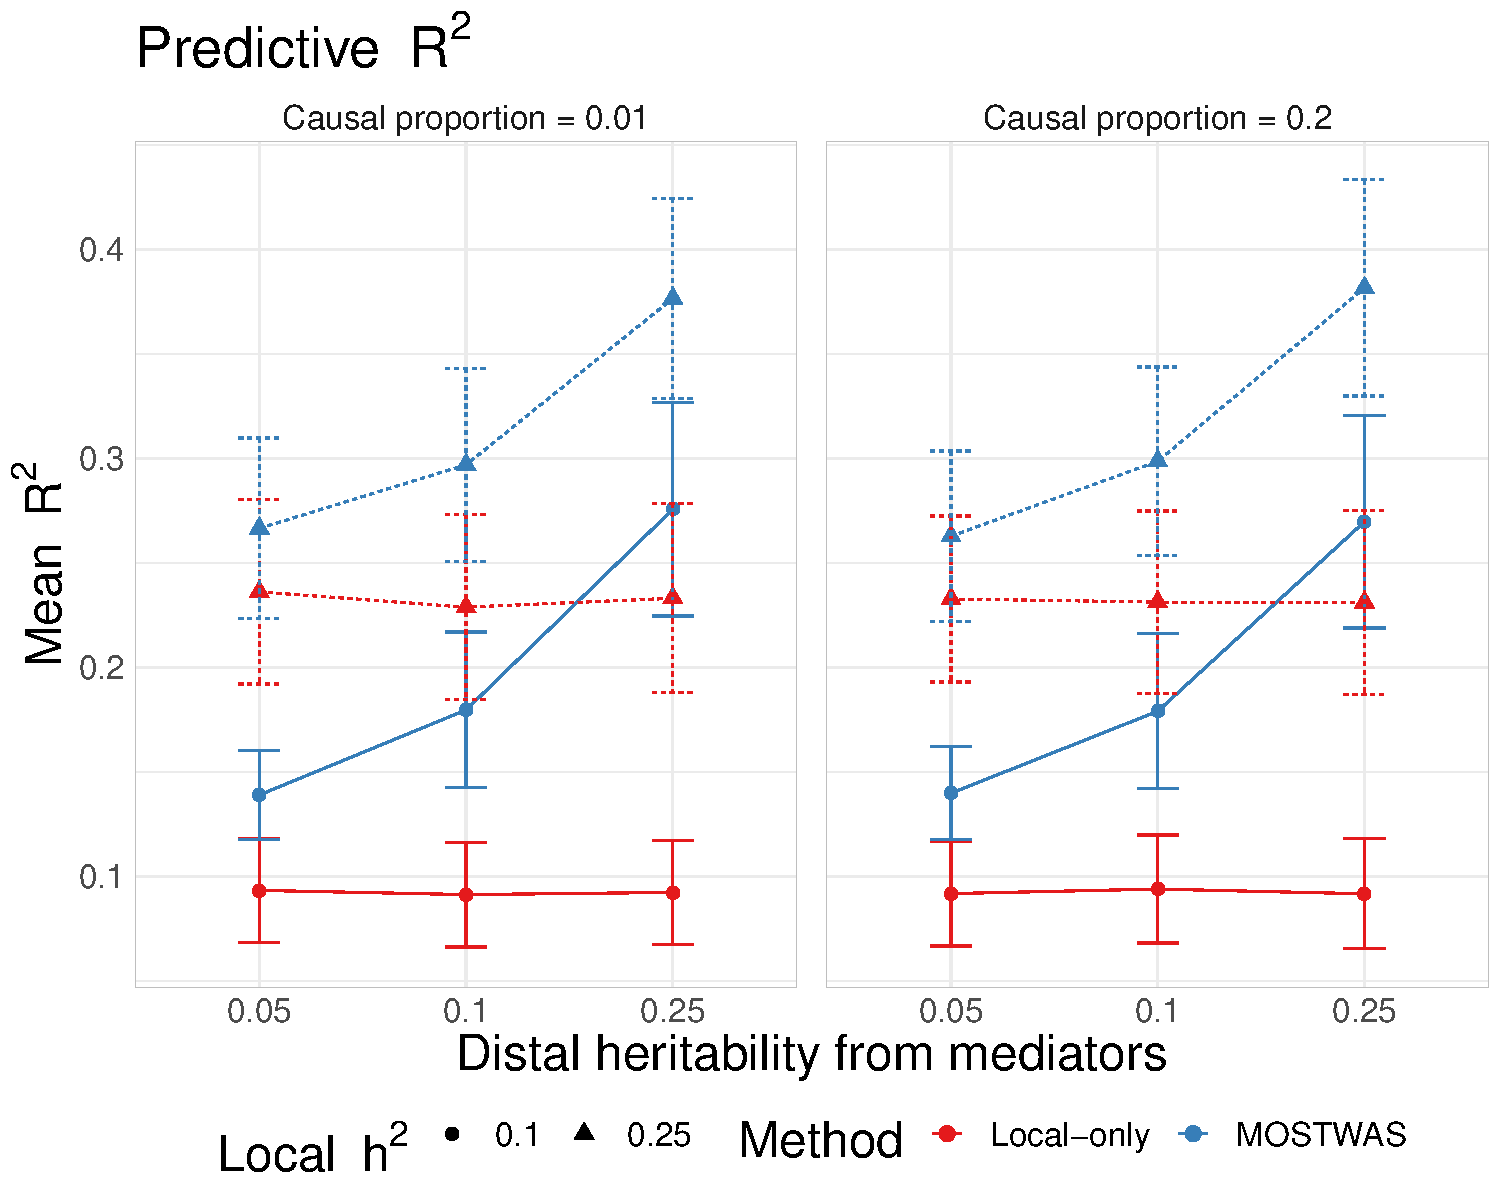
\includegraphics[width=\textwidth]{figures/ch4_suppfig1.pdf}
    \caption{\emph{Comparison of predictive $R^2$ in simulations.}
    Mean adjusted $R^2$ across various local and distal expression
    heritabilities, trait heritabilities,
    and causal proportions using local-only (red)
    and the best MOSTWAS (blue) models. The error bars
    reflect a width of 1 standard deviation
    of the 1,000 simulated adjusted $R^2$ values.}
    \label{fig:ch4_suppfig1}
\end{figure}
\end{center}

\begin{center}
\begin{figure}[!h]
    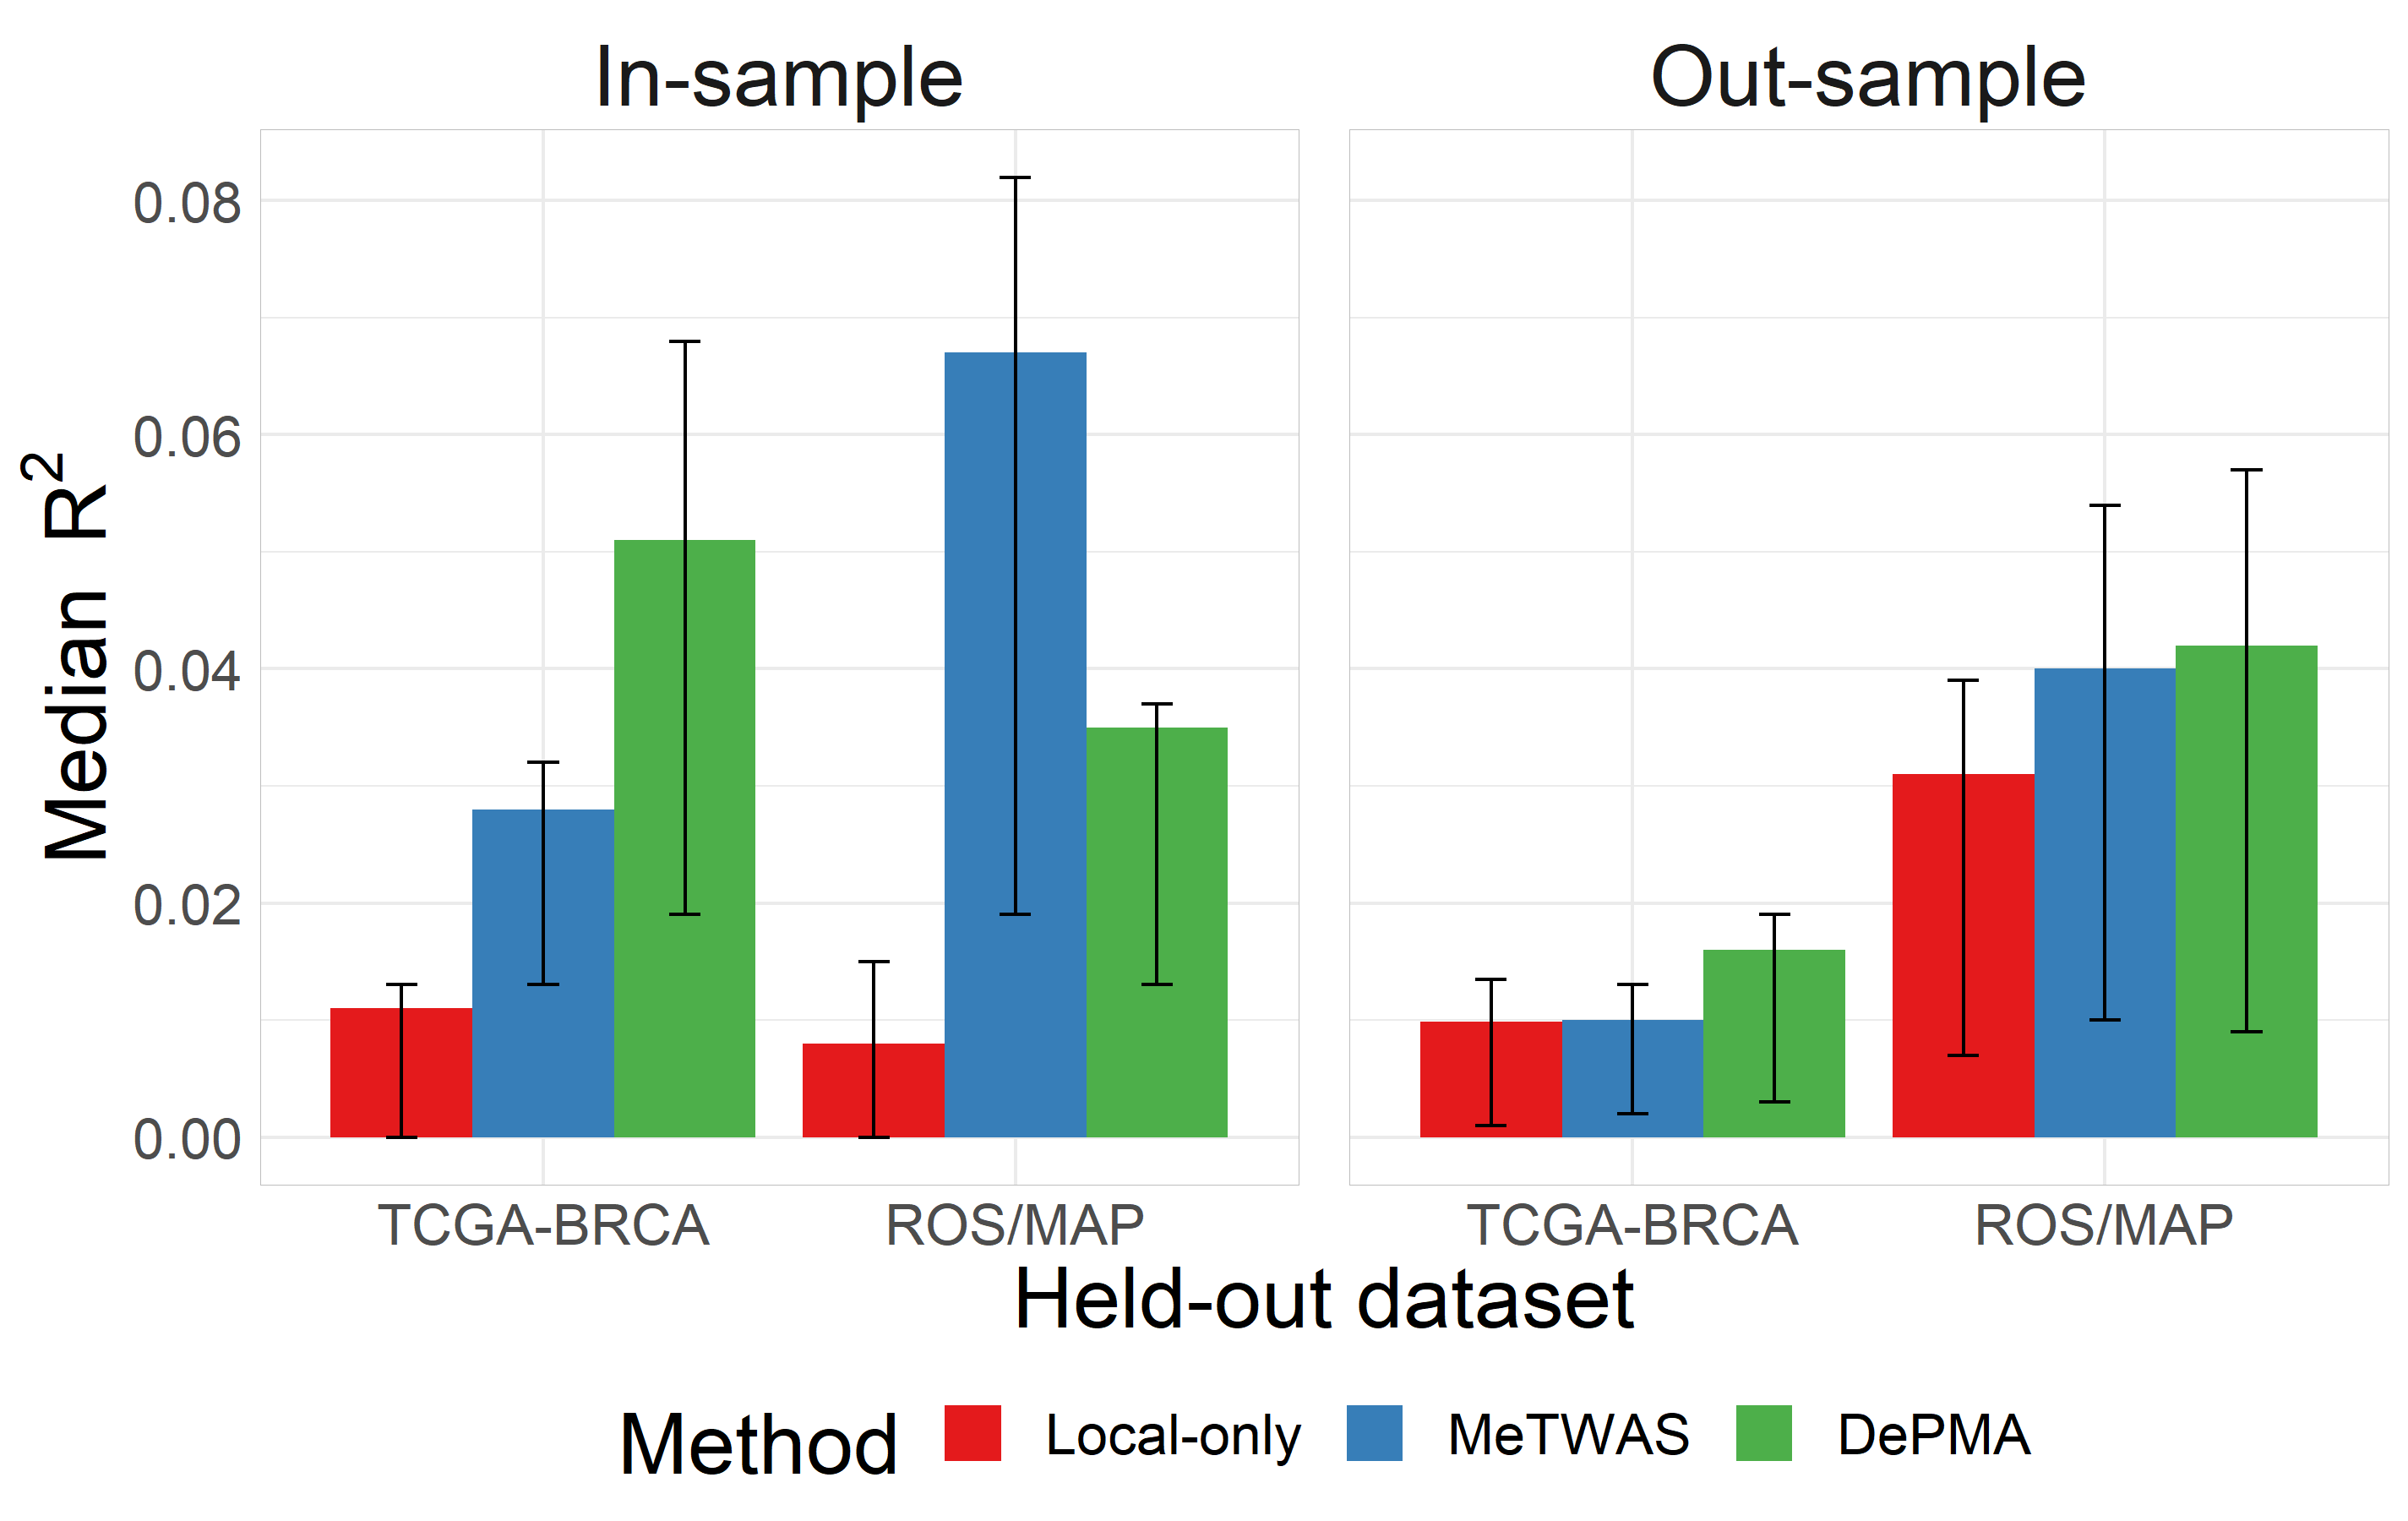
\includegraphics[width=\textwidth]{figures/ch4_suppfig3_5.png}
    \caption{\emph{Comparison of in-
    and out-sample predictive performance
    of local-only and MOSTWAS expression models.}
   Median predictive adjusted $R^2$
   for in-sample (left) and out-sample (right)
   performance in TCGA-BRCA and ROS/MAP
   expression models using local-only (red),
   MeTWAS (blue), and DePMA (green) modelling.
   The interval provided shows the 25\% and 75\%
   quartiles. Only genes with significant $h^2$
   at raw $P < 0.05$ are shown here.}
    \label{fig:ch4_suppfig3_5}
\end{figure}
\end{center}


\begin{center}
\begin{figure}[!h]
    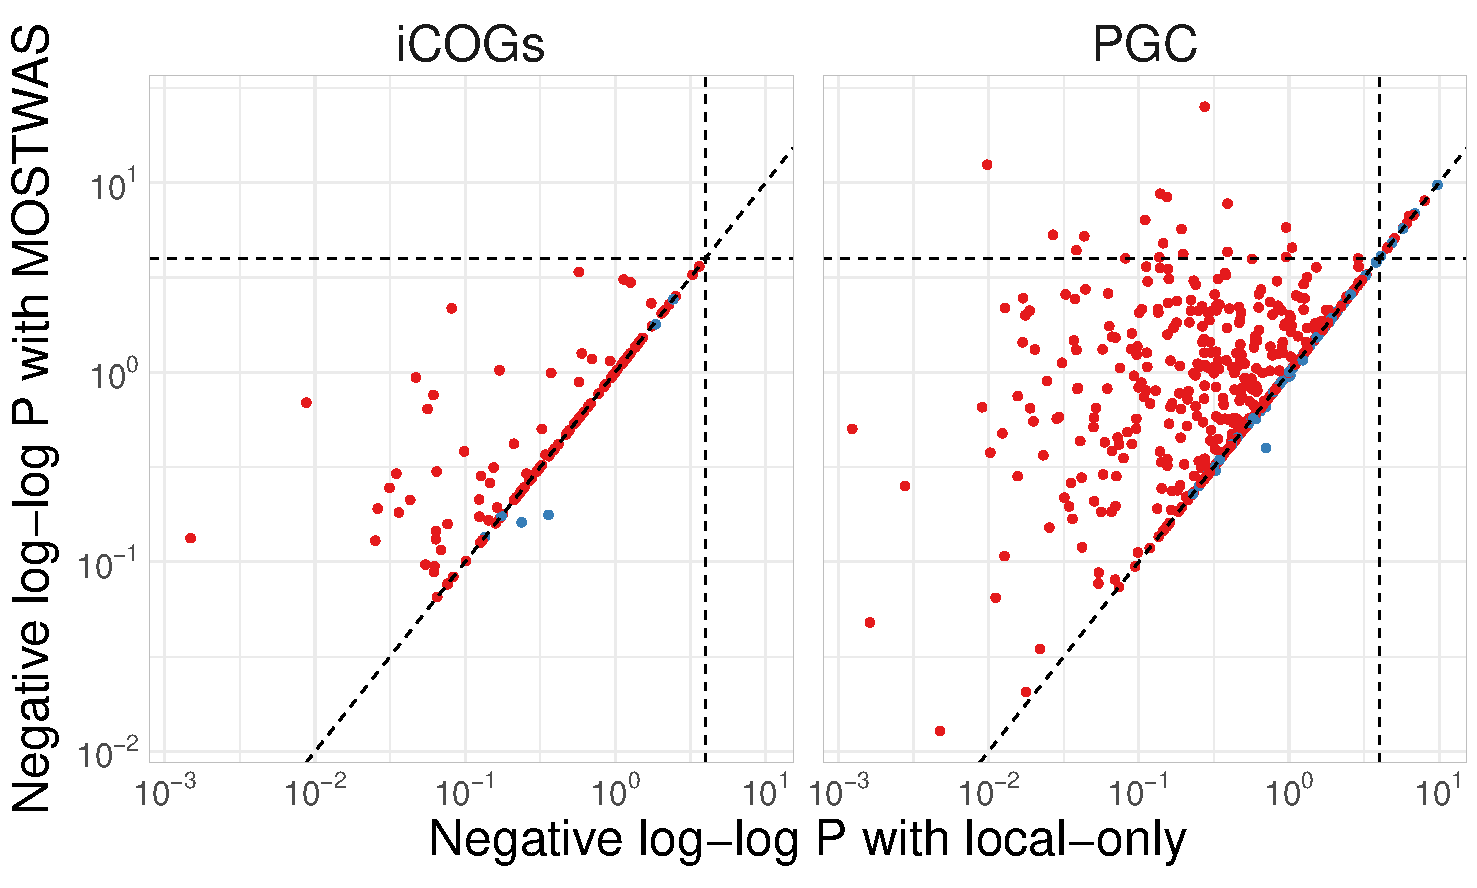
\includegraphics[width=\textwidth]{figures/ch4_suppfig2.pdf}
    \caption{\emph{Gene-trait associations in iCOGs
    and PGC using local-only and MOSTWAS models.} $-log_{10} P$-values of weighted
    burden gene-trait associations
    using iCOGs survival GWAS in European-ancestry
    women (left) and PGC MDD risk
    GWAS in predominantly 
    European-ancestry patients (right) 
    among genes that were predicted at cross-validation
    $R^2 \geq 0.01$ using both local-only
    and MOSTWAS models. The $X$- and $Y$-axes display
    the $-log_{10} P$-values for local-only
    and the best MOSTWAS model, respectively. Note
    that the scales of both axes are on a doubly logarithmic scale.
    Points are colored red if $P$-value
    of association is less than
    or equal using the MOSTWAS
    model. The horizontal and vertical reference lines indicate
    overall Bonferroni-corrected
    significance thresholds.}
    \label{fig:ch4_suppfig2}
\end{figure}
\end{center}

\pagebreak

\begin{landscape}
\begin{table}[]
\centering
\begin{tabular}{@{}ccccc@{}}
\toprule
\textbf{Gene} & \textbf{\begin{tabular}[c]{@{}c@{}}Cross-validation\\ $R^2$\end{tabular}} & \textbf{\begin{tabular}[c]{@{}c@{}}iCOGs $Z$-statistic \\ (Added-last $Z$)\end{tabular}} & \textbf{\begin{tabular}[c]{@{}c@{}}Top GWAS SNP location\\ ($P$)\end{tabular}} & \textbf{\begin{tabular}[c]{@{}c@{}}Permutation\\ FDR-adjusted $P$\end{tabular}} \\ \midrule
\textbf{C16orf13} & 0.019 & 4.51 (5.18) & \begin{tabular}[c]{@{}c@{}}Chr3:10720351\\ (0.13)\end{tabular} & 0.03 \\
\textbf{C9orf169} & 0.011 & 4.18 (3.97) & \begin{tabular}[c]{@{}c@{}}Chr19:44949849\\ (0.04)\end{tabular} & 0.03 \\
\textbf{CTRL} & 0.051 & 4.51 (3.88) & \begin{tabular}[c]{@{}c@{}}Chr10:2798136\\ (0.06)\end{tabular} & 0.03 \\
\textbf{DNAL4} & 0.013 & -3.94 (-4.57) & \begin{tabular}[c]{@{}c@{}}Chr22:38681840\\ (0.01)\end{tabular} & 0.04 \\
\textbf{LOC221710} & 0.014 & 5.34 (5.08) & \begin{tabular}[c]{@{}c@{}}Chr1:152983865\\ ($8.5 \times 10^{-4}$)\end{tabular} & 0.03 \\
\textbf{MAP3K6} & 0.021 & -4.10 (-4.00) & \begin{tabular}[c]{@{}c@{}}Chr1:27686314\\ (0.01)\end{tabular} & 0.05 \\
\textbf{MAP4K5} & 0.020 & 3.76 (1.26) & \begin{tabular}[c]{@{}c@{}}Chr14:50502944\\ ($1.3 \times 10^{-4}$)\end{tabular} & 0.03 \\
\textbf{NPAT} & 0.115 & -3.92 (-3.72) & \begin{tabular}[c]{@{}c@{}}Chr20:4217738\\ (0.02)\end{tabular} & 0.04 \\
\textbf{RPLP1} & 0.040 & -3.82 (-3.83) & \begin{tabular}[c]{@{}c@{}}Chr18:1592917\\ (0.18)\end{tabular} & $1.4 \times 10^{-4}$ \\
\textbf{SPATA5L1} & 0.042 & \begin{tabular}[c]{@{}c@{}}3.76 \\ (No distal SNPs in model)\end{tabular} & \begin{tabular}[c]{@{}c@{}}Chr15:45593323\\ (0.01)\end{tabular} & $1.4 \times 10^{-4}$ \\
\textbf{TXNRD2} & 0.047 & 3.91 (4.64) & \begin{tabular}[c]{@{}c@{}}Chr22:19735425\\ ($3.5 \times 10^{-3}$)\end{tabular} & 0.05 \\ \bottomrule
\end{tabular}
\caption{\emph{Summary statistics for 11
breast cancer-specific survival-associated loci identified
by MOSTWAS models.} TWAS associations with breast cancer survival 
from GWAS statistics from 
iCOGs with permutation test results and added-last $Z$-statistics. 
The top iCOGs GWAS SNP in the identified loci with its location and $P$-value are provided.}
\label{tbl:ch4_supptab11}
\end{table}
\end{landscape}

\pagebreak


\begin{landscape}
\begin{table}[]
\begin{tabular}{@{}cccccc@{}}
\toprule
\textbf{Gene} & \textbf{\begin{tabular}[c]{@{}c@{}}Z-statistic \\ (FDR-adjusted $P$)\end{tabular}} & \textbf{\begin{tabular}[c]{@{}c@{}}Cross-validation \\ $R^2$\end{tabular}} & \textbf{\begin{tabular}[c]{@{}c@{}}TOP GWAS SNP location \\ ($P$)\end{tabular}} & \textbf{\begin{tabular}[c]{@{}c@{}}Permutation\\ FDR-adjusted $P$\end{tabular}} & \textbf{\begin{tabular}[c]{@{}c@{}}Added last \\ FDR-adjusted $P$\end{tabular}} \\ \midrule
\textbf{ABCA7} & -1.82 (0.09) & 0.011 & \begin{tabular}[c]{@{}c@{}}Chr19:553,066 \\ (0.135)\end{tabular} & NA & NA \\
\textbf{ADAM10} & -1.25 (0.23) & 0.014 & \begin{tabular}[c]{@{}c@{}}Chr15:59,052,072 \\ ($1.68 \times 10^{-4}$)\end{tabular} & NA & NA \\
\textbf{APOE} & 2.82 (0.02) & 0.119 & \begin{tabular}[c]{@{}c@{}}Chr19:45,545,562 \\ ($3.0 \times 10^{-5}$)\end{tabular} & $5.0 \times 10^{-3}$ & 0.03 \\
\textbf{BIN1} & 1.91 (0.08) & 0.010 & \begin{tabular}[c]{@{}c@{}}Chr22:24,199,787 \\ ($8.53 \times 10^{-4}$)\end{tabular} & NA & NA \\
\textbf{CD2AP} & 1.52 (0.15) & 0.011 & \begin{tabular}[c]{@{}c@{}}Chr6:47,432,637 \\ ($1.23 \times 10^{-4}$)\end{tabular} & NA & NA \\
\textbf{CLU} & -2.41 (0.04) & 0.012 & \begin{tabular}[c]{@{}c@{}}Chr8:27,465,312 \\ ($1.33 \times 10^{-4}$)\end{tabular} & 0.83 & 0.44 \\
\textbf{FERMT2} & 2.13 (0.06) & 0.017 & \begin{tabular}[c]{@{}c@{}}Chr14:53,305,626 \\ ($1.38 \times 10^{-4}$)\end{tabular} & NA & NA \\
\textbf{MEF2C} & 2.20 (0.06) & 0.016 & \begin{tabular}[c]{@{}c@{}}Chr5:88,359,039 \\ (0.020)\end{tabular} & NA & NA \\
\textbf{PLCG2} & -2.48 (0.04) & 0.010 & \begin{tabular}[c]{@{}c@{}}Chr16:81,879,218 \\ (0.037)\end{tabular} & 0.66 & 0.07 \\
\textbf{SORL1} & 2.91 (0.02) & 0.043 & \begin{tabular}[c]{@{}c@{}}Chr11:121,446,813 \\ (0.032)\end{tabular} & 0.04 & $4.5 \times 10^{-3}$ \\
\textbf{ZCWPW1} & -4.56 ($6.1 \times 10^{-5}$) & 0.018 & \begin{tabular}[c]{@{}c@{}}Chr7:100,435,157 \\ (0.074)\end{tabular} & 0.03 & $1.3 \times 10^{-5}$ \\ \bottomrule
\end{tabular}
\caption{\emph{Summary statistics for known
Alzheimer's risk-associated loci identified
by MOSTWAS models.} TWAS associations (weighted
$Z$-score and FDR-adjusted\cite{Benjamini1995}
$P$-value) with late-onset
Alzheimer's risk from GWAS statistics from IGAP\cite{Lambert2013Meta-analysisDisease}.
The top IGAP GWAS SNP in the identified loci with its location and $P$-value are provided.
For the 6 loci with significant
TWAS associations, the FDR-adjusted $P$-value
for the
follow-up
distal SNP added last test is provided.}
\label{tbl:ch4_supptab2}
\end{table}
\end{landscape}

\pagebreak

\begin{center}
\begin{figure}[!h]
\centering
    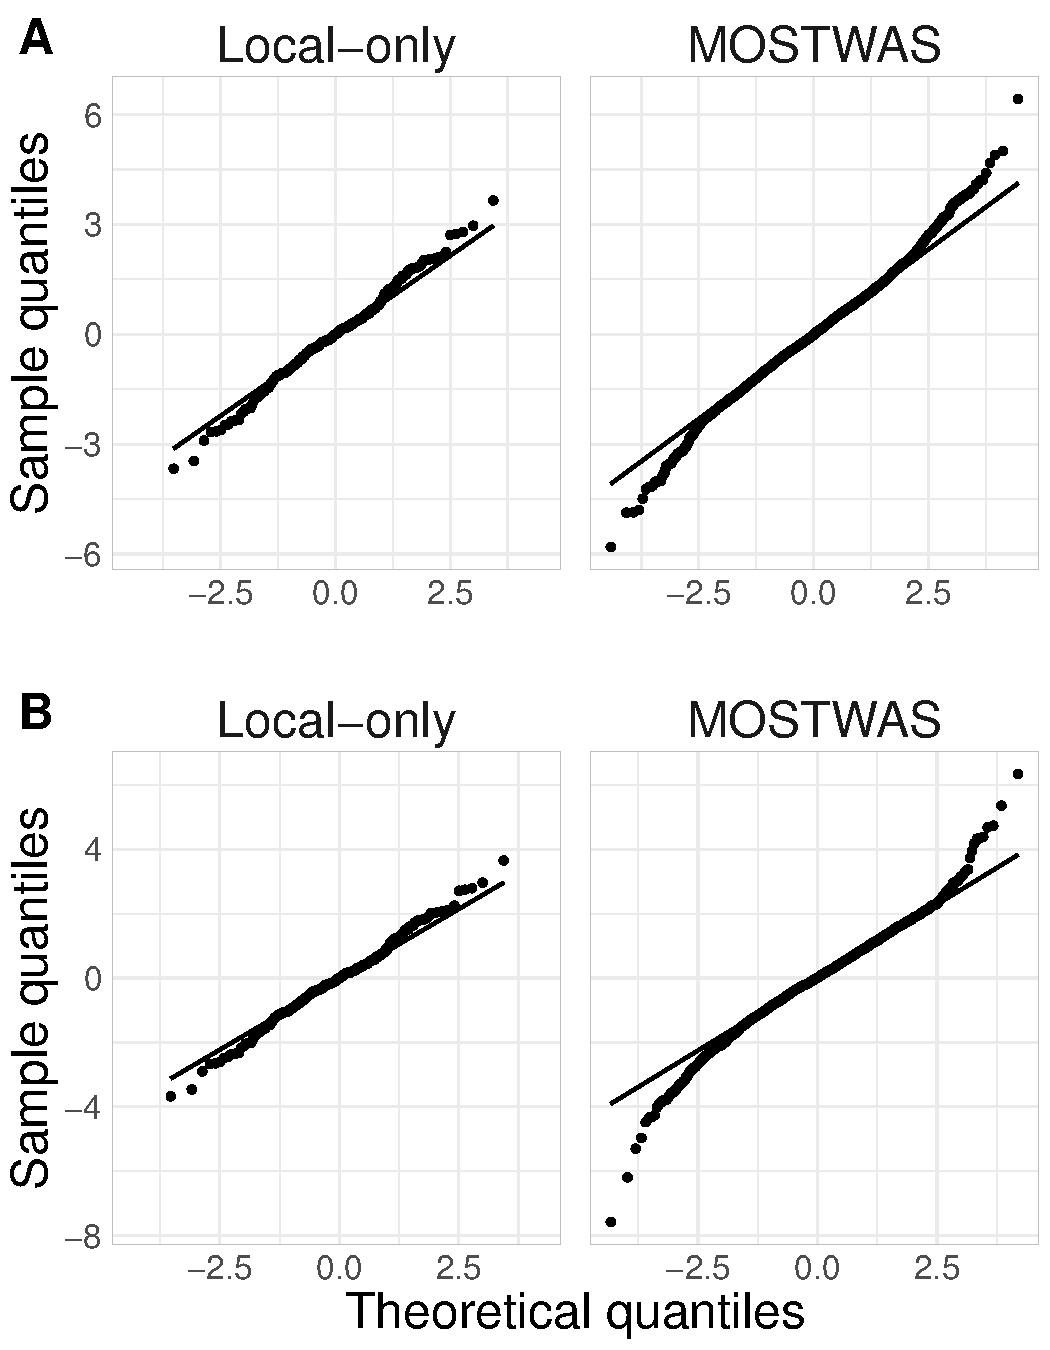
\includegraphics[width=.8\textwidth]{figures/ch4_suppfig3.pdf}
    \caption{\emph{Comparison of QQ-plots
    from TWAS associations.} QQ-plots
    from TWAS for breast 
    cancer-specific survival in iCOGs (A) 
    and MDD in PGC (B)
    with local-only models (left)
    and MOSTWAS (right)}
    \label{fig:ch4_suppfig3}
\end{figure}
\end{center}


\pagebreak


\begin{table}[]
\centering
\begin{tabular}{@{}ccccc@{}}
\toprule
\multicolumn{1}{l}{\textbf{Gene}} & \textbf{\begin{tabular}[c]{@{}c@{}}Cross-validation\\ $R^2$\end{tabular}} & \textbf{\begin{tabular}[c]{@{}c@{}}PGC $Z$-statistic \\ (UKBB $Z$)\end{tabular}} & \textbf{\begin{tabular}[c]{@{}c@{}}Top GWAS SNP location\\ ($P$)\end{tabular}} & \textbf{\begin{tabular}[c]{@{}c@{}}Permutation\\ FDR-adjusted $P$\end{tabular}} \\ \midrule
\textbf{ADAD2} & 0.050 & 5.89 (4.16) & \begin{tabular}[c]{@{}c@{}}Chr5:35,639,107\\ ($4.05 \times 10^{-3}$)\end{tabular} & $3.5 \times 10^{-5}$ \\
\textbf{CACNA2D3} & 0.033 & 3.41 (2.88) & \begin{tabular}[c]{@{}c@{}}Chr7:12,268,243\\ ($1.27 \times 10^{-2}$)\end{tabular} & 0.046 \\
\textbf{FAM43B} & 0.035 & -4.03 (-2.85) & \begin{tabular}[c]{@{}c@{}}Chr2:73,148,399\\ ($2.09 \times 10^{-2}$)\end{tabular} & 0.028 \\
\textbf{MGC29506} & 0.022 & 3.51 (5.54) & \begin{tabular}[c]{@{}c@{}}Chr5:139,536,922\\ ($1.48 \times 10^{-3}$)\end{tabular} & $3.5 \times 10^{-5}$ \\
\textbf{OR8U1} & 0.022 & -3.19 (-4.21) & \begin{tabular}[c]{@{}c@{}}Chr11:56,676,947\\ ($4.90 \times 10^{-5}$)\end{tabular} & 0.049 \\
\textbf{SYT1} & 0.015 & -5.58 (-3.16) & \begin{tabular}[c]{@{}c@{}}Chr7:12,269,417\\ ($1.29 \times 10^{-2}$)\end{tabular} & 0.040 \\
\textbf{YJEFN3} & 0.010 & 5.82 (7.22) & \begin{tabular}[c]{@{}c@{}}Chr7:12,276,011\\ ($1.35 \times 10^{-2}$)\end{tabular} & 0.038 \\ \bottomrule
\end{tabular}
\caption{\emph{Summary statistics for 7
MDD risk-associated loci identified
by MOSTWAS models.} TWAS associations with major depressive disorder from GWAS statistics from Psychiatric Genomics Consortium that were replicated with GWAX summary statistics in UK Biobank. The top PGC GWAS SNP in the identified loci with its location and $P$-value are provided.}
\label{tbl:ch4_supptab3}
\end{table}

\begin{center}
\begin{figure}[!h]
    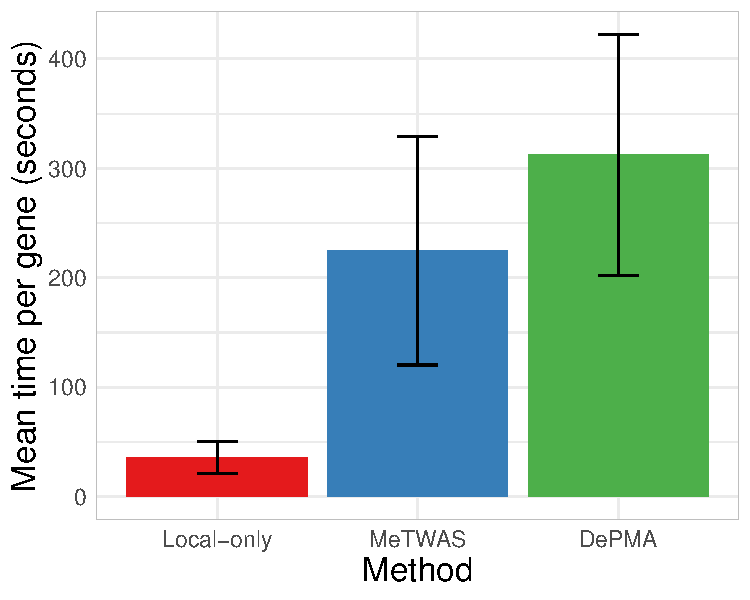
\includegraphics[width=.9\textwidth]{figures/ch4_suppfig0.pdf}
    \caption{\emph{Comparison of computation times
    between local-only and MOSTWAS modelling.}
    Mean and standard deviation of per-gene computation time
    across 50 randomly selected genes in TCGA-BRCA.
    Computations here were done with a 24-core,
    3.0 GHz processor.}
    \label{fig:ch4_suppfig0}
\end{figure}
\end{center} 

\pagebreak
  
%This is where your bibliography is generated. Make sure that your .bib file is actually called library.bib
\bibliography{library}
  
%This defines the bibliographies style. Search online for a list of available styles.
\bibliographystyle{unsrt2abbrv}


\end{document}
